\section{Au-delà du modèle standard}\label{chapter-MS-MSSM-section-BSM}
Le modèle standard souffre ainsi de lacunes malgré ses prédictions précises.
Des modèles sont développés afin de les combler, ils sont dits \og au-delà \fg{} du modèle standard (BSM, \emph{Beyond Standard Model}).
Un de ces modèles BSM est la supersymétrie (SUSY).
La section~\ref{chapter-MS-MSSM-section-BSM-subsec-SUSY} présente la SUSY et motive l'introduction d'un second doublet de Higgs.
La SUSY est en effet un cas particulier de modèle à deux doublets de Higgs (2HDM, \emph{2 Higgs Doublets Model}).
Les 2HDM sont abordés dans la section~\ref{chapter-MS-MSSM-section-BSM-subsec-dbl_H_dbl}.
Puis, le modèle le plus simple de SUSY, l'extension supersymétrique minimale du modèle standard (MSSM, \emph{Minimal Supersymmetric extension of Standard Model}), est présenté section~\ref{chapter-MS-MSSM-section-BSM-subsec-MSSM}.
\subsection{Supersymétrie}\label{chapter-MS-MSSM-section-BSM-subsec-SUSY}
La supersymétrie (SUSY)~\cite{susy_golfand,susy_wess,MARTIN_1998} introduit une nouvelle symétrie entre fermions et bosons.
Ces deux types de particules ne sont plus indépendants, ce sont des saveurs, ou manifestations, d'un champ quantique plus complexe.
Du fait de cette symétrie,
à chaque particule du modèle standard correspond une nouvelle particule ou \og superpartenaire \fg.
Les fermions du modèle standard ont des superpartenaires de spin entier, \ie\ des bosons, les \og sfermions \fg.
Les bosons du modèle standard ont des superpartenaires de spin demi-entier, \ie\ des fermions, les \og bosinos \fg.
Une particule et son superpartenaire ont les mêmes nombres quantiques à l'exception de leurs spins.
\par De nouvelles interactions sont possibles, dans lesquelles les nombres baryonique $B$ et leptonique $L$ ne sont pas conservés et $B-L$ non plus.
Le proton est alors instable, ce qui n'est pas observé expérimentalement.
Une nouvelle symétrie est ainsi introduite afin de restaurer la conservation de $B-L$, la parité $R$.
L'opérateur de parité $R$ est défini comme
\begin{equation}
P_R = (-1)^{3(B-L)-2s}
\end{equation}
où $s$ correspond au spin de la particule.
La parité $R$ est égale à $1$ pour les particules du modèle standard,
$-1$ pour leurs superpartenaires.
La conservation de cette nouvelle parité permet non seulement de garder le proton stable, mais rend également stable la particule supersymétrique de plus basse masse, notée LSP (\emph{Lightest Supersymmetric Particle}).
\par La SUSY permet résoudre de nombreuses lacunes du modèle standard.
Elle permet par exemple d'unifier trois forces fondamentales (électromagnétique, faible et forte).
Dans la section~\ref{chapter-MS-MSSM-section-formalisme-subsec-EW}, l'unification des forces électromagnétique et faible est déjà réalisée.
Toutefois, la force électrofaible et la force forte ne semblent pas s'unifier à haute énergie.
Or, les interactions avec les superpartenaires introduits par la SUSY modifient le comportement des constantes de couplage des trois forces fondamentales de manière à les unifier à haute énergie.
La SUSY propose également un candidat pour la matière noire dans le cas où la LSP est de charge électrique nulle, il peut être un neutralino ou un sneutrino.
De plus, la SUSY permet de résoudre le problème de l'ajustement fin.
La divergence quadratique de la masse du Higgs est naturellement supprimée par les diagrammes à boucles des superpartenaires dont les contributions ont des signes opposés à celles des particules, les fermions ayant des contributions positives et les bosons des contributions négatives~\cite{Higgs_hunter_guide}.
\par Toutefois, il est impossible de mettre en place la SUSY sans un second doublet de Higgs.
Dans le modèle standard, la masse des quarks d'isospin faible haut est obtenue dans la section~\ref{chapter-MS-MSSM-section-formalisme-subsec-Higgs_mechanism-subsubsec-fermions} à l'aide du conjugué de charge du doublet de Higgs.
Cependant, le potentiel supersymétrique contenant les termes de Yukawa, nécessaires à l'obtention des masses des fermions, n'autorise pas l'utilisation de ce conjugué afin de donner une masse aux quarks d'isospin faible haut~\cite{Nagashima_BSM}.
Un second doublet de Higgs, couplé aux fermions d'isospin faible haut, doit nécessairement être introduit~\cite{Nagashima_BSM,Higgs_hunter_guide}.
La SUSY est donc un cas particulier de modèle à deux doublets de Higgs.
\subsection{Modèles à deux doublets de Higgs}\label{chapter-MS-MSSM-section-BSM-subsec-dbl_H_dbl}
Dans les modèles à deux doublets de Higgs (2HDM),
le doublet de Higgs du modèle standard $\phi$ défini par~\eqref{eq-chapter-MS-MSSM-section-formalisme-subsec-Higgs_mechanism-SM_Higgs_doublet}
est remplacé par deux doublets $\phi_1$ et $\phi_2$
et
le potentiel de Higgs~\eqref{eq-chapter-MS-MSSM-section-formalisme-subsec-Higgs_mechanism-SM_Higgs_potential}
par
le potentiel scalaire le plus général possible brisant spontanément $SU(2)_L \times U(1)_Y$~\cite{Higgs_hunter_guide,Higgs_hunter_guide_errata},
\begin{multline}
V(\phi_1,\phi_2)
= \lambda_1 \left(\phi_1^\dagger\phi_1 - \frac{1}{2} v_1^2\right)^2
+ \lambda_2 \left(\phi_2^\dagger\phi_2 - \frac{1}{2} v_2^2\right)^2
\\
+ \lambda_3 \left[ \left(\phi_1^\dagger\phi_1 - \frac{1}{2} v_1^2\right) + \left(\phi_2^\dagger\phi_2 - \frac{1}{2} v_2^2\right) \right]^2
+ \lambda_4 \left[ (\phi_1^\dagger\phi_1)(\phi_2^\dagger\phi_2) - (\phi_1^\dagger\phi_2)(\phi_2^\dagger\phi_1) \vphantom{\frac{1}{2}}\right]
\\
+ \lambda_5 \left[ \Re(\phi_1^\dagger\phi_2) - \frac{1}{2} v_1v_2\cos\xi \right]^2
+ \lambda_6 \left[ \Im(\phi_1^\dagger\phi_2) - \frac{1}{2} v_1v_2\sin\xi \right]^2
\\
+ \lambda_7 \left[ \Re(\phi_1^\dagger\phi_2) - \frac{1}{2} v_1v_2\cos\xi \right]\left[ \Im(\phi_1^\dagger\phi_2) - \frac{1}{2} v_1v_2\sin\xi \right]
\mend[,]
\label{eq-chapter-MS-MSSM-section-BSM-subsec-dbl_H_dbl-Higgs_potential}
\end{multline}
où $\lambda_i$, $i\in\set{1,\ldots,7}$ et $\xi$ sont des paramètres du modèle à valeurs réelles.
Dans le cas de la SUSY, $\lambda_5=\lambda_6$.
Le dernier terme de~\eqref{eq-chapter-MS-MSSM-section-BSM-subsec-dbl_H_dbl-Higgs_potential} peut être éliminé en redéfinissant les phases des champs scalaires.
Dans le cas $\sin\xi\neq0$, le secteur de Higgs du modèle viole la symétrie $CP$,
ce cas est abordé dans la section~\ref{chapter-MS-MSSM-section-BSM-subsec-CPV}.
Le minimum du potentiel ainsi construit est tel que
\begin{equation}
\average{\phi_1}_0 = \frac{1}{\sqrt{2}} \begin{pmatrix}
0\\v_1
\end{pmatrix}
\msep
\average{\phi_2}_0 = \frac{1}{\sqrt{2}} \begin{pmatrix}
0\\v_2 \eexp{\im\xi}
\end{pmatrix}
\mend
\end{equation}
\par Il est possible de définir, à ce stade, une variable importante dans la suite, le rapport des condensats des doublets de Higgs dans le vide,
\begin{equation}
\tan\beta = \frac{\average{\phi_2}_0}{\average{\phi_1}_0} = \frac{v_2}{v_1}
\label{eq-tan_beta-2HDM}
\end{equation}
avec $0\leq\beta\leq\pi/2$.
Il est aussi possible de définir
\begin{equation}
v^2 = v_1^2+v_2^2
\mend
\end{equation}
\par De ce formalisme découle l'existence de cinq bosons de Higgs massifs,
\begin{align}
&
\text{deux Higgs chargés:}
&
\Higgspm &= - \phi_1^\pm \sin\beta + \phi_2^\pm \cos\beta
\msep&
m_{\Higgspm}^2 &= \frac{1}{2} \lambda_4 v^2
\mend[,]
\\
&
\text{un Higgs pseudo-scalaire:}
&
\HiggsA &= \sqrt{2}\left(-\Im(\phi_1^0)\sin\beta+\Im(\phi_2^0)\cos\beta\right)
\msep&
m_{\HiggsA}^2 &= \frac{1}{2} \lambda_6 v^2
\mend[,]
\end{align}
ainsi que deux bosons de Higgs scalaires neutres dont les champs quantiques sont mélangés par la matrice
\begin{equation}
\mathcal{M} = \frac{1}{2} \begin{pmatrix}
4v_1^2 (\lambda_1+\lambda_3) + v_2^2\lambda_5 & (4\lambda_3+\lambda_5)v_1v_2 \\
(4\lambda_3+\lambda_5)v_1v_2 & 4v_2^2 (\lambda_2+\lambda_3) + v_1^2\lambda_5
\end{pmatrix}
\mend
\end{equation}
Ces deux bosons de Higgs sont
\begin{align}
\higgs &= \sqrt{2}\left(-\Re(\phi_1^0-v_1/\sqrt{2})\sin\alpha+\Re(\phi_2^0-v_2/\sqrt{2})\cos\alpha\right)
\mend[,]
\\
\Higgs &= \sqrt{2}\left(\Re(\phi_1^0-v_1/\sqrt{2})\cos\alpha+\Re(\phi_2^0-v_2/\sqrt{2})\sin\alpha\right)
\mend[,]
\end{align}
où l'angle de mélange $\alpha$ s'obtient par
\begin{equation}
\sin 2\alpha = \frac{2\mathcal{M}_{12}}{\sqrt{(\mathcal{M}_{11}-\mathcal{M}_{22})^2+4\mathcal{M}_{12}^2}}
\msep
\cos 2\alpha = \frac{\mathcal{M}_{11}-\mathcal{M}_{22}}{\sqrt{(\mathcal{M}_{11}-\mathcal{M}_{22})^2+4\mathcal{M}_{12}^2}}
\end{equation}
avec $-\pi/2\leq\alpha\leq0$
et
dont les masses à l'ordre le plus bas s'expriment, avec $m_{\higgs} \leq m_{\Higgs}$,
\begin{equation}
m_{\higgs,\Higgs}^2 = \frac{1}{2} \left( \mathcal{M}_{11} + \mathcal{M}_{22} \mp \sqrt{(\mathcal{M}_{11}-\mathcal{M}_{22})^2+4\mathcal{M}_{12}^2} \right)
\mend
\end{equation}
Enfin, $v$ est fixée par la masse du \Wboson,
\begin{equation}
m_{\Wboson} = \frac{1}{2}vg_I
\label{eq-2HDM_W_mass}
\mend
\end{equation}
\par Le 2HDM ainsi construit possède 6 paramètres libres:
\begin{itemize}
\item $m_{\higgs}$, $m_{\Higgs}$, $m_{\HiggsA}$, $m_{\Higgspm}$ les masses des bosons de Higgs;
\item $\tan\beta$ le rapport des condensats des doublets de Higgs dans le vide;
\item $\alpha$ l'angle de mélange des Higgs.
\end{itemize}
\par Ce modèle peut être affiné par les observations expérimentales.
Par exemple, le changement de saveur par courant neutre (FCNC, \emph{Flavor-Changing Neutral Currents}), n'est pas observé expérimentalement.
Afin d'être compatible avec ce fait expérimental~\cite{Higgs_hunter_guide},
\begin{itemize}
\item soit les masses des bosons de Higgs sont élevées, de l'ordre du \SI{}{\TeV}, supprimant ainsi suffisamment le FCNC pour rester dans les limites observées;
\item soit tous les fermions portant une même charge électrique ne sont couplés qu'à un seul doublet de Higgs au plus.
\end{itemize}
La masse du boson de Higgs du modèle standard n'étant pas de l'ordre du \SI{}{\TeV}, la seconde option est choisie.
\begin{wraptable}{R}{.5\textwidth}
\centering
\begin{tabular}{rccc}
\toprule
Couplage avec & \higgs & \Higgs & \HiggsA \\
\midrule
Bosons vecteurs & \!$\sin(\beta-\alpha)$\! & \!$\cos(\beta-\alpha)$\! & $0$\\
Fermions hauts & $\displaystyle \frac{\cos\alpha}{\sin\beta}$ & $\displaystyle \frac{\sin\alpha}{\sin\beta}$ & \!$\cot\beta$\! \\
Fermions bas & $\displaystyle \frac{-\sin\alpha}{\cos\beta}$ & $\displaystyle \frac{\cos\alpha}{\cos\beta}$ & \!$\tan\beta$\! \\
\bottomrule
\end{tabular}
\caption[Couplages des bosons de Higgs neutres.]{Couplages des bosons de Higgs neutres des modèles de type~II par rapport aux couplages du boson de Higgs du modèle standard~\cite{Higgs_hunter_guide}.}
\label{tab-Higgs_couplings_2HDM}
\end{wraptable}
\par
Dans les modèle de type~I, les fermions ne sont pas couplés à $\phi_1$, mais le sont à $\phi_2$.
Dans le cas des modèles de type~II, les fermions d'isospin faible bas sont couplés à $\phi_1$ et ceux d'isospin faible haut à $\phi_2$.
Les intensités des couplages des fermions et des bosons avec \higgs, \Higgs\ et \HiggsA\ ainsi obtenues, par rapport à celles avec le boson de Higgs du modèle standard, sont présentées dans le tableau~\ref{tab-Higgs_couplings_2HDM}.
%En particulier, le couplage du boson de Higgs du modèle standard, \higgs, est modifié et une mesure précise de ses couplages aux autres particules est un test de ce type de modèles.
\par Les modèles à deux doublets de Higgs sont donc une extension du modèle standard ajoutant une nouvelle physique, en particulier l'existence de nouveaux bosons de Higgs.
Ils doivent nécessairement être introduits dans les modèles supersymétriques pour que ceux-ci respectent les observations expérimentales.
\subsection{Extension supersymétrique minimale du modèle standard}\label{chapter-MS-MSSM-section-BSM-subsec-MSSM}
L'extension supersymétrique minimale du modèle standard ou MSSM~\cite{mssm_fayet1,mssm_fayet2}
est le modèle le plus simple permettant d'introduire la SUSY tout en étant compatible avec les observations expérimentales à ce jour.
Dans le MSSM, les deux doublets de Higgs s'expriment en fonction de $\phi_1$ et $\phi_2$ introduits dans la section~\ref{chapter-MS-MSSM-section-BSM-subsec-dbl_H_dbl} comme~\cite{Higgs_hunter_guide}
\begin{equation}
\Higgs_d
=
\begin{pmatrix}
{\phi_1^0}^* \\ -\phi_1^-
\end{pmatrix}
\msep
\Higgs_u
=
\begin{pmatrix}
\phi_2^+ \\ \phi_2^0
\end{pmatrix}
\mend
\label{eq-chapter-MS-MSSM-section-BSM-Higgs_doublets}
\end{equation}
L'expression du potentiel de Higgs général des 2HDM~\eqref{eq-chapter-MS-MSSM-section-BSM-subsec-dbl_H_dbl-Higgs_potential} devient
\begin{align}
V(\Higgs_d,\Higgs_u)
&
=
\mu_d^2\Higgs_d^\dagger\Higgs_d
+
\mu_u^2\Higgs_u^\dagger\Higgs_u
-
\mu^2 (\Higgs_d\wedge\Higgs_u+\text{h.c.})
\nonumber\\
&\hphantom{=}
+
\frac{g_I^2+g_Y^2}{8} (\Higgs_d^\dagger\Higgs_d-\Higgs_u^\dagger\Higgs_u)^2
+
\frac{g_I^2}{2} (\Higgs_d^\dagger\Higgs_u)^2
\end{align}
en posant~\cite{Higgs_hunter_guide,Higgs_hunter_guide_errata,Nagashima_BSM}
\vspace{-.5\baselineskip}\par\noindent
\begin{subequations}
\noindent
\begin{minipage}[c]{.49\textwidth}
\begin{align}
\lambda_2 &= \lambda_1 \mend[,]\\
\lambda_3 &= \frac{1}{8} (g_I^2+g_Y^2)-\lambda_1 \mend[,]\\
\lambda_4 &= 2\lambda_1 - \frac{1}{2} g_Y^2 \mend[,]\\
\lambda_5 &= \lambda_6 = 2\lambda_1 - \frac{1}{2}(g_I^2+g_Y^2) \mend[,]
\end{align}
\end{minipage}
\hfill
\begin{minipage}[c]{.49\textwidth}
\begin{align}
\mu_d^2 &= \mu^2\tan\beta - \frac{1}{2} m_{\Zboson}^2 \cos(2\beta) \mend[,]\\
\mu_u^2 &= \mu^2\cot\beta + \frac{1}{2} m_{\Zboson}^2 \cos(2\beta) \mend[,]\\
\mu^2 &= -\frac{1}{2}v_1v_2(g_I^2+g_Y^2-4\lambda_1)
\mend
\end{align}
\end{minipage}
\end{subequations}
\vspace{.5\baselineskip}\par\noindent
Afin d'assurer la stabilité du vide, le potentiel ne doit pas pouvoir être infiniment bas, ce qui implique $\mu_u^2+\mu_d^2 > 2\mu^2$ si $\abs{\phi_1^0}=\abs{\phi_2^0}$.
La brisure spontanée de symétrie donnant leurs masses aux bosons de l'interaction faible est présente si $\mu^4>\mu_u^2 \mu_d^2$.
Alors, les condensats dans le vide des deux doublets de Higgs sont
\begin{equation}
\average{\Higgs_d}_0 = \frac{1}{\sqrt{2}} \begin{pmatrix}v_1 \\ 0 \end{pmatrix}
\msep
\average{\Higgs_u}_0 = \frac{1}{\sqrt{2}} \begin{pmatrix} 0\\ v_2 \end{pmatrix}
\mend
\end{equation}
\par Les masses des bosons de Higgs s'expriment alors à l'ordre le plus bas
\begin{align}
m_{\HiggsA}^2 &= \mu^2 (\tan\beta+\cot\beta) = \frac{2\mu^2}{\sin 2\beta}
\mend[,] \label{eq-mA-MSSM}\\
m_{\Higgspm}^2 &= m_{\HiggsA}^2+m_{\Wboson}^2
\mend[,] \label{eq-mHpm-MSSM}\\
m_{\higgs,\Higgs}^2 &= \frac{1}{2} \left( m_{\HiggsA}^2+m_{\Zboson}^2 \mp \sqrt{(m_{\HiggsA}^2+m_{\Zboson}^2)^2-4m_{\HiggsA}^2m_{\Zboson}^2\cos^2 2\beta} \right)
\mend[,] \label{eq-mH0-MSSM}
\end{align}
et l'angle de mélange des Higgs scalaires neutres vérifie
\begin{equation}
\cos 2\alpha = - \frac{m_{\HiggsA}^2-m_{\Zboson}^2}{m_{\Higgs}^2-m_{\higgs}^2} \cos 2\beta
\msep
\sin 2\alpha = - \frac{m_{\HiggsA}^2+m_{\Zboson}^2}{m_{\Higgs}^2-m_{\higgs}^2} \sin 2\beta
\mend
\label{eq-Higgs_mixing_angle_MSSM}
\end{equation}
Enfin, la masse du \Wboson\ vérifie toujours~\eqref{eq-2HDM_W_mass} et celle du \Zboson\ peut être exprimée en fonction des paramètres du MSSM. Ainsi,
\begin{equation}
m_{\Wboson} = \frac{1}{2}vg_I
\Leftrightarrow
m_{\Wboson}^2 = \frac{1}{4}v^2g_I^2
\msep
m_{\Zboson}^2 = \frac{\mu_d^2 - \mu_u^2 \, \tan^2\beta}{\tan^2\beta-1}
\mend
\end{equation}
\par À l'ordre le plus bas, les masses des bosons de Higgs dépendent donc seulement de deux paramètres libres, $m_{\HiggsA}$ et $\tan\beta$ défini par~\eqref{eq-tan_beta-2HDM}.
Il est à noter que l'équation~\eqref{eq-mH0-MSSM} implique l'existence d'un boson de Higgs neutre de masse inférieure à $m_{\Zboson}=\SI{91.19}{\GeV}$.
Toutefois, ceci n'est vrai qu'à l'ordre le plus bas.
La prise en compte des corrections radiatives change les expressions de ces masses, en particulier celles dues au quark top et à son superpartenaire le stop.
La masse du boson de Higgs léger est ainsi modifiée selon~\cite{Nagashima_BSM}
\begin{equation}
m_{\higgs}^2 \to m_{\higgs}^2 + \delta m_{\higgs}^2
\simeq m_{\Zboson}^2
+ \frac{3 m_{\quarkt}^4}{2 \pi^2 v^2} \left[ \ln\frac{m_S^2}{m_{\quarkt}^2} + \frac{X_t^2}{m_S^2}\left(1-\frac{X_t^2}{12 m_S^2} \right) \right]
\end{equation}
où
\begin{equation}
X_t = A_t - \mu\cot\beta
\end{equation}
est le paramètre de mélange du stop,
avec $A_t$ sa constante de couplage aux Higgs,
et
\begin{equation}
m_S = \sqrt{m_{\squarkt_1}m_{\squarkt_2}}
\mend
\end{equation}
est l'échelle d'énergie de la SUSY, définie comme la moyenne géométrique des masses des stops.
Il existe en effet deux états propres de masse pour ces particules,
$\squarkt_1$ et $\squarkt_2$,
mélanges des stops de chiralité droite et gauche.
La présence de nombreux paramètres libres du MSSM mène à proposer des scénarios dans lesquels les paramètres intervenant dans les corrections d'ordres supérieurs sont fixés~\cite{Carena_2013,Bagnaschi_2019}.
Il ne reste alors que deux paramètres libres, $m_{\HiggsA}$ et $\tan\beta$.
Les valeurs des masses corrigées de \higgs, \Higgs\ et \Higgspm\ sont tracées sur la figure~\ref{fig-Higgs_corrected_masses_as_fct_of_mA_and_tanbeta} en fonction de $m_{\HiggsA}$ pour $\tan\beta=3$ et $30$ dans le cas de mélange maximal du stop avec $m_{\squarkt}=\SI{2}{\TeV}$ et les autres paramètres de la SUSY fixés à \SI{1}{\TeV}~\cite{Nagashima_BSM}.
Ainsi, pour $m_{\HiggsA} \lesssim \SI{125}{\GeV}$, \Higgs\ joue le rôle du modèle standard et il existe un Higgs léger.
Pour $m_{\HiggsA} \gtrsim \SI{125}{\GeV}$, \higgs\ joue le rôle du modèle standard et les bosons de Higgs supplémentaires sont de masses plus élevées.
Dans ce cas, $m_{\Higgs}\simeq m_{\HiggsA}$.
\begin{figure}[h]
\centering
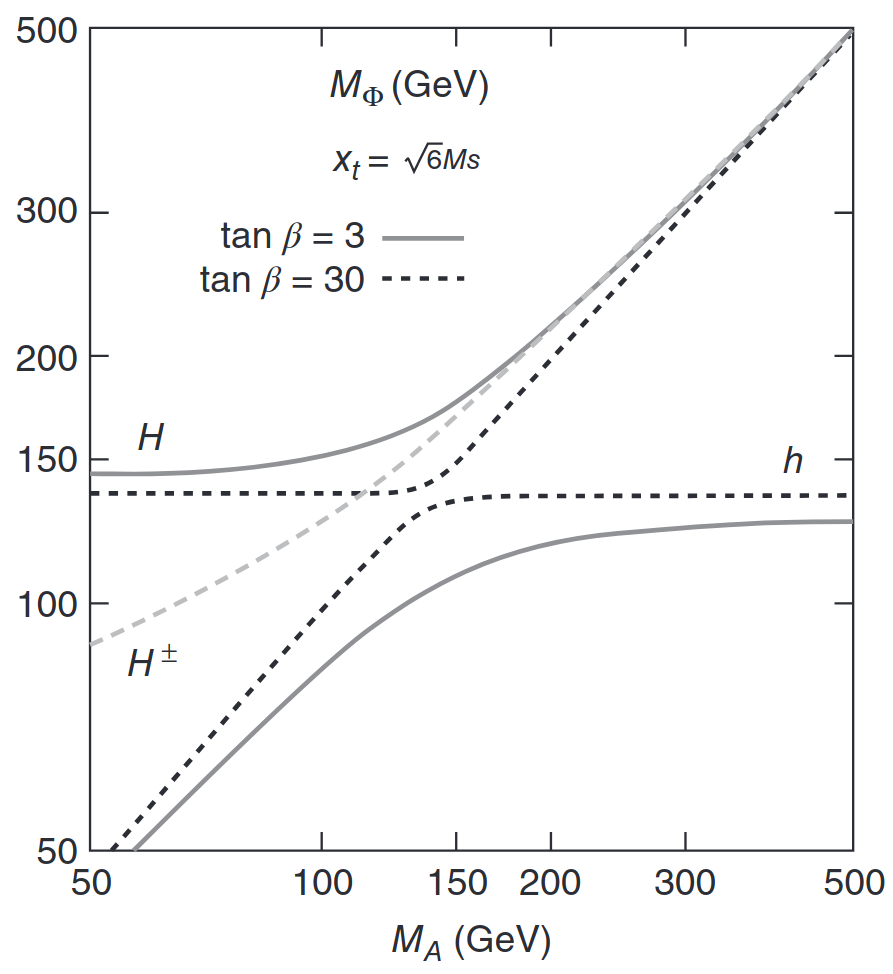
\includegraphics[width=.45\textwidth]{\PhDthesisdir/plots_and_images/from_Nagashima_BSM/fig_1-9.tex}
\caption[Masses des bosons de Higgs du MSSM.]{Masses des bosons de Higgs du MSSM en fonction de $m_{\HiggsA}$ pour $\tan\beta=3$ et $30$ dans le cas de mélange maximal du stop avec $m_{\squarkt}=\SI{2}{\TeV}$ et les autres paramètres de la SUSY fixés à \SI{1}{\TeV}~\cite{Nagashima_BSM}.}
\label{fig-Higgs_corrected_masses_as_fct_of_mA_and_tanbeta}
\end{figure}
\par Les particules du MSSM et leurs superpartenaires sont résumés dans le tableau~\ref{tab-ptcs_and_superpartners}.
Un test expérimental est possible par la recherche d'un signal correspondant aux bosons de Higgs supplémentaires, ce qui fait l'objet de cette thèse.
L'étude de la phénoménologie de ces bosons de Higgs, présentée ci-après, permet de déterminer les conditions favorables à la recherche d'un tel signal.
\begin{table}[h]
\centering
\begin{tabular}{cccccccc}
\toprule
\multicolumn{4}{c}{Particules} & \multicolumn{4}{c}{Superpartenaires}\\
\cmidrule(lr){1-4}\cmidrule(lr){5-8}
Type & Spin & Particules & Symboles & Type & Spin & Particules & Symboles \\
\midrule
\multirow{2}{*}{Fermions} & \multirow{2}{*}{$\dfrac{1}{2}$} & quarks & \quark &
\multirow{2}{*}{Sfermions} & \multirow{2}{*}{$0$} & squarks & \squark \\
 &  & leptons & $\ell$ &
 &  & sleptons & $\tilde{\ell}$ \\
\cmidrule(lr){1-8}
\multirow{5}{*}{Bosons} & \multirow{4}{*}{$1$} & gluon & \gluon &
\multirow{5}{*}{Bosinos} & \multirow{5}{*}{$\dfrac{1}{2}$} & gluino & \gluino \\
 & & bosons \Wbosonpm & \Wbosonplus, \Wbosonminus &
 & & winos & \sWbosonplus, \sWbosonminus \\
 & & photon & \photon &
 & & photino & \photino \\
 & & boson \Zboson & \Zboson &
 & & zino & \sZboson \\
 & $0$ & Higgs & \higgs, \Higgs, \HiggsA, \Higgspm &
 & & Higgsinos & $\tilde{h}$, $\tilde{H}$, $\tilde{A}$, $\tilde{H}^\pm$  \\
\bottomrule
\end{tabular}
\caption[Particules et leurs superpartenaires.]{Particules et leurs superpartenaires. La présence de plusieurs bosons de Higgs est justifiée par la nécessité d'un second doublet de Higgs. Ce formalisme est décrit dans la section~\ref{chapter-MS-MSSM-section-BSM-subsec-dbl_H_dbl}.}
\label{tab-ptcs_and_superpartners}
\end{table}
\subsection{Violation de $CP$ avec les bosons de Higgs}\label{chapter-MS-MSSM-section-BSM-subsec-CPV}
L'asymétrie matière-antimatière ne peut être expliquée par la seule violation de $CP$ de l'interaction faible.
Or, une violation de $CP$ dans les couplages de Yukawa est possible lorsque le paramètre $\xi$ de l'équation~\eqref{eq-chapter-MS-MSSM-section-BSM-subsec-dbl_H_dbl-Higgs_potential} vérifie $\sin\xi\neq0$.
\par
Les termes de Yukawa s'écrivent en général, pour un boson de Higgs $\Phi$,
\begin{equation}
\Lcal_\text{Yukawa}
= - \frac{m\sqrt{2}}{v} \left( \cos(\varphi) \bar{\psi} \Phi \psi + \sin(\varphi) \bar{\psi} \im\gamma^5 \Phi \psi \right)
\end{equation}
avec $\varphi$ l'angle de mélange $CP$ de $\Phi$.
Lorsque $\varphi=0$, $\Phi$ est $CP$-pair, \ie\ scalaire avec un nombre quantique $J^{CP}=0^{++}$.
Pour $\varphi=\frac{\pi}{2}$, $\Phi$ est $CP$-impair, \ie\ pseudo-scalaire avec un nombre quantique $J^{CP}=0^{+-}$.
Pour toutes les autres valeurs de $\varphi$, l'état est mixte et permet une violation de $CP$.
\par
Dans le MSSM sans violation de $CP$, les états propres de masse des bosons de Higgs neutres sont également des états propres de $CP$.
Ainsi
\higgs\ et \Higgs\ sont $CP$-pairs
et
\HiggsA\ est $CP$-impair.
Avec violation de $CP$,
les états propres de masse sont des états mixtes de $CP$.
Afin de les distinguer de \higgs, \Higgs\ et \HiggsA,
ils sont notés, par masse croissante,
$\Higgs_1$, $\Higgs_2$ et $\Higgs_3$.
%Dans le cadre de la recherche de bosons supplémentaires de haute masse,
%le rôle du boson de Higgs du modèle standard \higgs\ est pris par $\Higgs_1$.
\par
Les sections qui suivent traitent du cas sans violation de $CP$.
Le cas avec violation correspond, dans le cadre de ma thèse, au passage
$\set{\higgs,\Higgs,\HiggsA} \to \set{\Higgs_1,\Higgs_2,\Higgs_3}$.